
\subsection{Mission Study and Management Plan  }
\label{sec:management}

\vspace{-0.05in}

\subsubsection{Study Plan}

\vspace{-0.05in}

The mission study is open to the entire CMB community and includes 75 scientists. 
To gain maximum benefit from \planck , LiteBIRD, and CORE we invited international members to participate. 
The work is organized into Working Groups (WG); see 
Figure~\ref{fig:management}. Working groups are led by members of the study's Executive Committee, 
as listed in the Figure. Although Figure~\ref{fig:management} suggests distinct boundaries between the 
WGs we expect and encourage significant overlap and feedback. It is not practical to enumerate all 
the interdependencies. 
\begin{figure}[ht!]
\vspace{-0.1in}
%\hspace{-0.1in}
\parbox{3.5in}{\centerline {
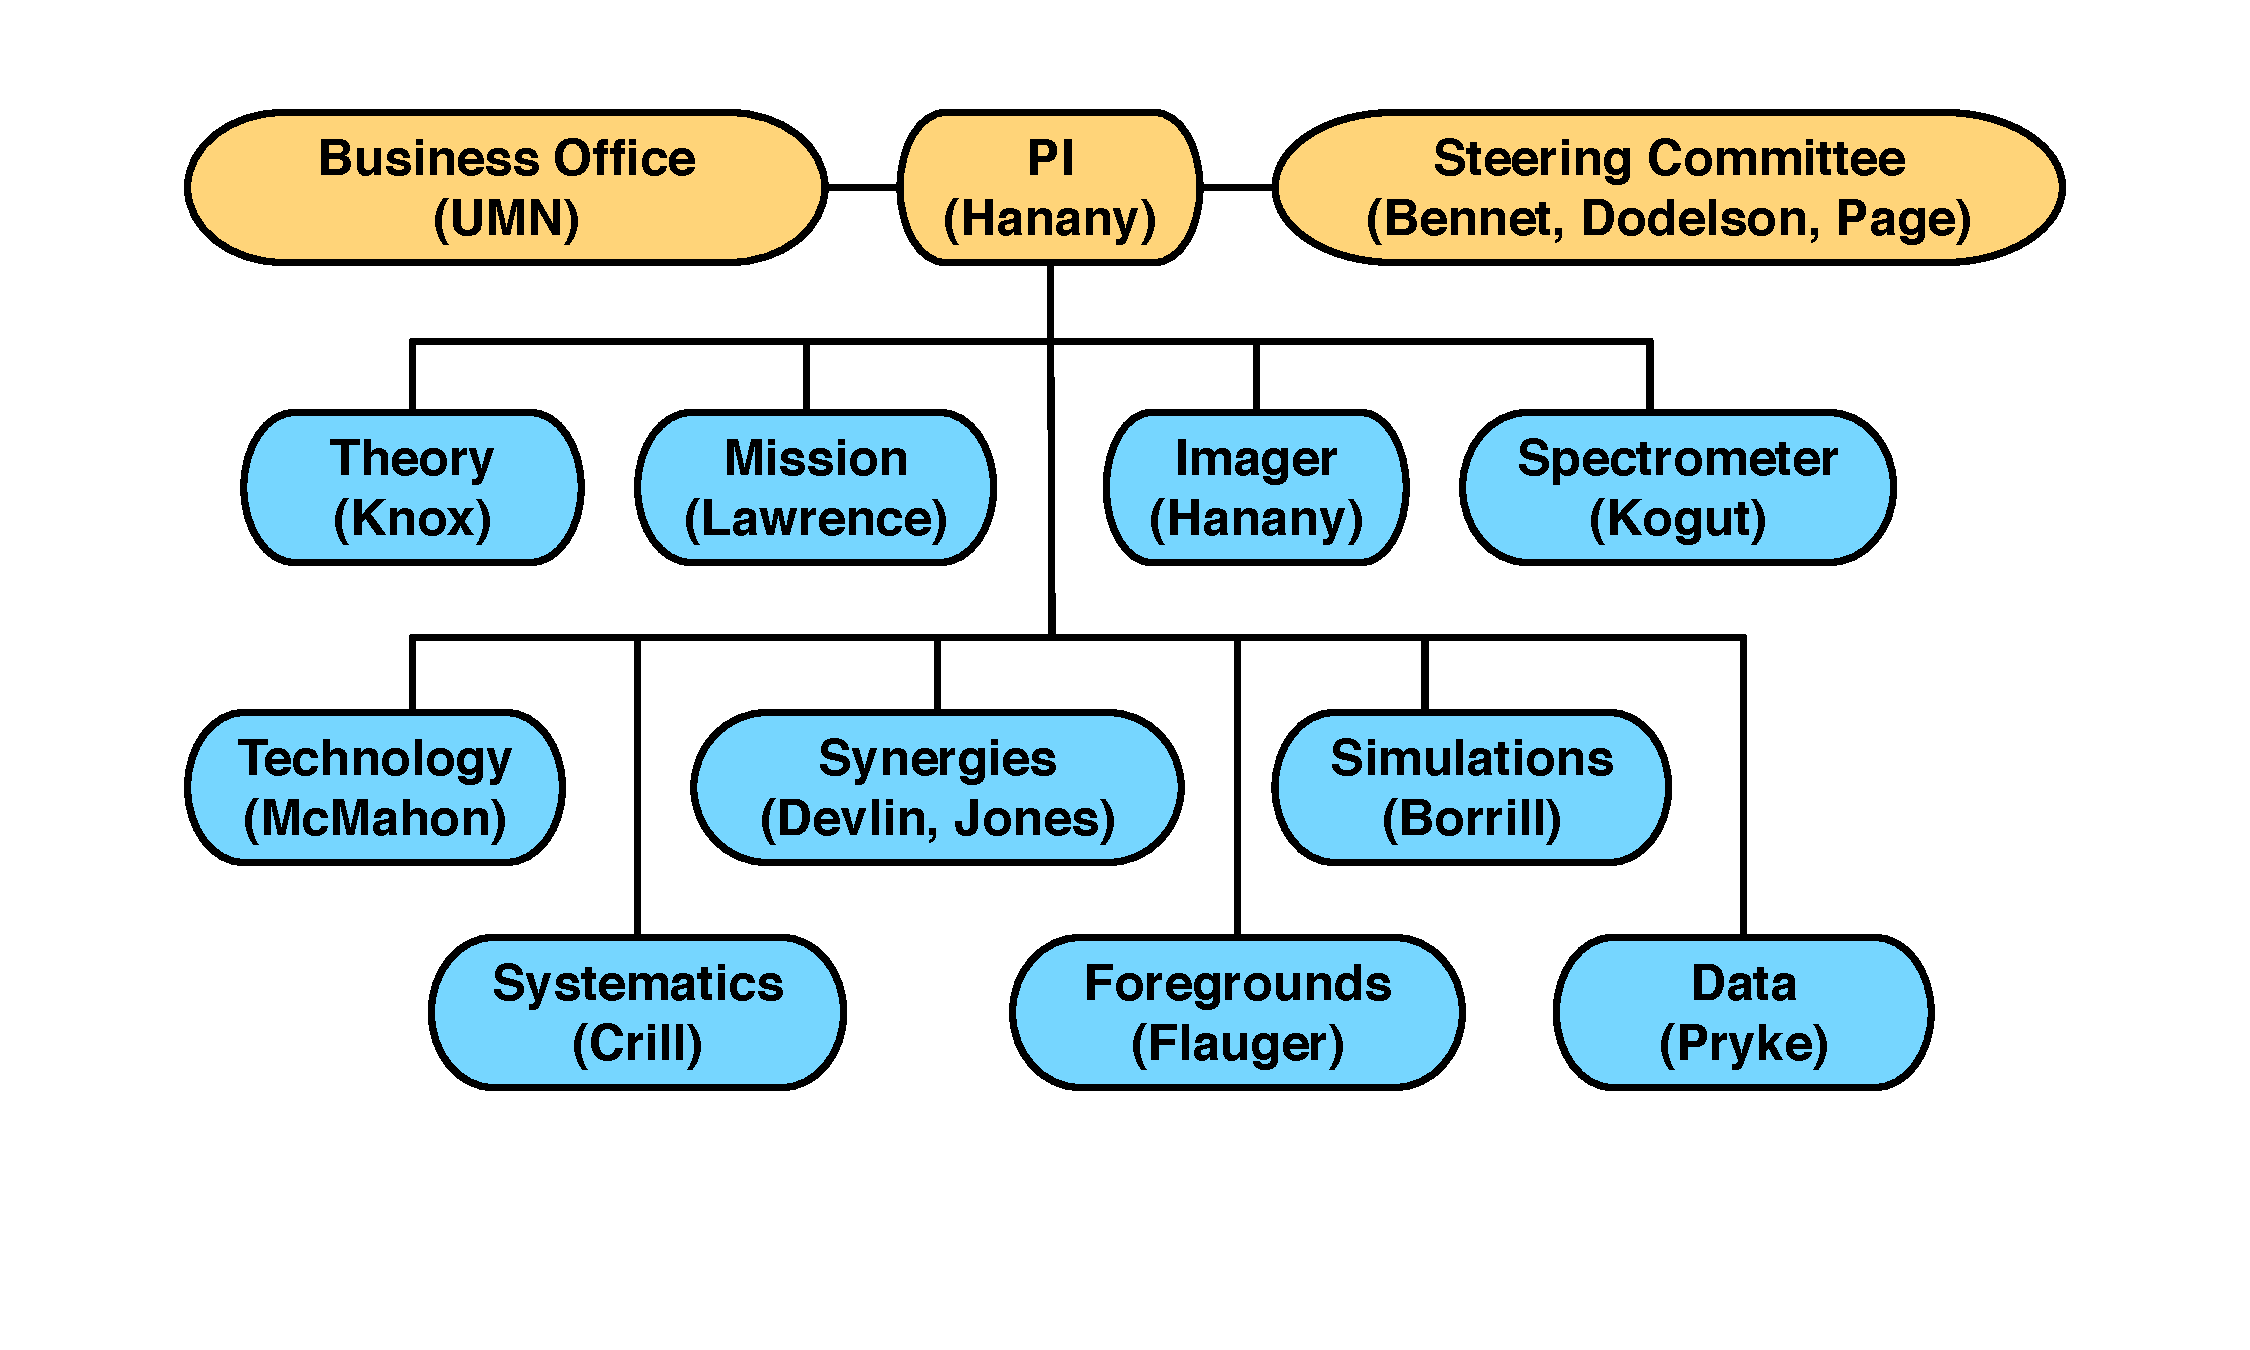
\includegraphics[width=3.1in]{Figures/OrgChart_namesV3} } }
\hspace{0.05in}
%\end{center}
\parbox{2.8in}{
\caption{ \small \setlength{\baselineskip}{0.95\baselineskip}
Management structure of the CMB Probe. A steering committee advises the PI. The study is led by the PI 
through an Executive Committee. Each member of the committee is in charge of a specific Working Group (blue boxes). Significant overlap and feedback is expected between the working groups.  Participation in the Working Groups is open to all members of the CMB community. 
\label{fig:management} } }
\vspace{-0.15in}
\end{figure}

The study will be carried out through intra- and inter-WG teleconferences; mission design teleconference with JPL engineers; 
mission design meetings at JPL; and a community workshop that is described in more detail below.  
A central activity that cuts across several of the WGs is the development and use of 
a `Mission Performance Simulator'. The mission performance simulator takes as input a particular 
instrument configuration (e.g number of detectors, frequencies, resolutions), sky observing pattern, models of 
sky emission (including CMB and foregrounds), and systematic effects. It generates detector timestreams that 
are used to make maps. The maps can be analyzed for their astrophysical content. 

We now describe the work of each of the WGs and, where appropriate, lay out responsibilities for 
elements of the mission performance simulator. \\
$\bullet$ {\bf Theory (Knox)} \hspace{0.1in} This WG will survey, summarize, and prioritize the set of 
science goals for the Probe.  Given input on target frequency bands, assumptions about foregrounds, 
instrument systematics, and instrument noise levels the group will generate forecasts for the impact of 
the Probe�s products and their significance to physics and astrophysics. This group 
will also investigate which other astrophysical data sets are most suitable for cross-correlation analysis 
with the Probe's data. \\
$\bullet$ {\bf Mission and connection with JPL (Lawrence)} \hspace{0.1in} The Mission WG is responsible 
for defining the overall mission architecture including telescope implementation, cooling, telemetry, mass, 
power, and cost. We are requesting that engineering and costing session be conducted with JPL. 
Charles Lawrence, Chief Scientist of the Astronomy, Physics, and Space Technology Directorate at JPL, and 
the \planck\ US PI, will lead this WG. \\
$\bullet$ {\bf Imager (Hanany) and Spectrometer (Kogut)} \hspace{0.1in} The imager and spectrometer WGs will 
translate the science goals to mission requirements and to nominal designs. The designs will include telescopes 
of various configurations, focal planes with several candidate detector technologies and readout schemes, optical 
elements, and cooling strategies. These groups will similarly consider 
the options for spectrometers.  Both groups will interact frequently with JPL
the Mission WG. The WG will consider an imager-only design, a spectrometer-only design, and
a combined instrument.  This group will provide focal plane configurations for the mission performance simulator. \\
$\bullet$ {\bf Technology (McMahon)} \hspace{0.1in} 
This working group will provide technical input to the team designing the mission and instruments.  It will 
assess the most appropriate technologies given the implementation of the mission and identify technologies that are in need 
of development. A central topic of assessment will be the technical readiness and possible implementation of a
polarization modulator.  \\
$\bullet$ {\bf Space / Sub-Orbital Synergy (Devlin, Jones)} \hspace{0.1in} By the time the \ac{CMB} probe is likely to fly,
significant advances will have been made on the ground. This is true regardless of the state of the proposed CMB-S4
effort, and even more so should funding for S4 becomes available soon. This WG will assess and recommend the 
most appropriate design parameters such that the data sets from the Probe and sub-orbital measurements complement each other. 
Pertinent questions include: to what extent should the aperture size of the Imaging Probe rely on delensing capabilities provided by 
high resolution measurements from the ground? What is the optimal resolution of a space-based mission from the point 
of view of providing foreground subtraction capabilities to sub-orbital missions? What is an optimal overlap in $\ell$-space
coverage? Does the design of a spectrometer depend on the specifics of data available from sub-orbital measurements? 
We are planning a community workshop to address these question, including forming a community consensus on the 
question of the need for a space mission if CMB-S4 is funded. \\
$\bullet$ {\bf Data Analysis and Exploitation (Pryke)} \hspace{0.1in}
The full sky nature, the broad frequency coverage, and the high  sensitivity of the CMB-Probe will generate a legacy data 
set surpassing that of \planck 's. This WG will plan for  the extraction of cosmological and astrophysical 
products from the Probe's data. This includes exploring optimal implementation of component separation techniques, 
of combining sub-orbital CMB data with the Probe's, and of cross-correlating with 
data at other wavelengths. The WG will assess whether specific synergies suggest preferring some mission parameter values 
over others. The group will use outputs of the mission performance simulator. \\
%The group will also survey possible sources of systematic uncertainties that are introduced during 
%the analysis process and how these can be addressed during mission 
%design, implementation, and data analysis. 
$\bullet$ {\bf Systematics (Crill)} \hspace{0.1in} This WG will identify sources of systematic effects,
evaluate their approximate magnitude, and will construct the tools to integrate the these 
systematic effects into the mission performance simulator. Examples include frequency band 
mismatches, differential gains, and sidelobes.  The WG will explore mitigation 
of systematic errors by design, for example implementing modulation 
schemes and modulator technologies, and mitigation by analysis techniques.   \\
$\bullet$ {\bf Foregrounds (Flauger) } \hspace{0.1in} This WG will construct foregrounds models that encompass all the 
known and expected emission complexities. The models will be informed by data and physical inputs 
and will include, for example, spatial variations of the spectral dependence, decorrelation between frequencies, and departures 
from a simple modified black body law for 
Galactic dust~\cite{draine_fraisse_2009,Draine:2012zu,planck2015_x,planck2016_l,planck2016_xxix,Vansyngel:2016fbn}. 
The models will be used as part of the Mission Performance Simulator. 
The WG will also study, develop, test, and recommend methods for component separation including 
those used with \planck ~\cite{planck2015_ix}. \\
$\bullet$ {\bf Simulations (Borrill)} \hspace{0.1in} This WG will be in charge of building and running 
the mission performance simulator. It is based on the massively parallel tools built for the Planck Full 
Focal Plane simulations~\cite{plank2015_xii_focalplane}. The simulations 
will use the high performance computing resources available to the CMB community at the 
DOE's National Energy Research Scientific Computing (NERSC) Center at Lawrence Berkeley National 
Laboratory. 

\vspace{-0.18in}

\subsubsection{Mission Study Timeline}

\vspace{-0.05in}

The study will be conducted in three broad phases with several months overlap to allow for the non-linear
nature of the progression: Mission Definition; Mission Implementation; Report Writeup. \\
{\bf Mission Definition: 3/2017 - 12/2017} \hspace{0.1in} The primary output of this period 
is a set of mission requirements that will feed into 
the Mission Implementation phase. To achieve a set of mission requirements we will use the 
mission performance simulator to iterate over various angular resolutions, focal plane configurations,  
detector noise properties and progressively more complex foreground and systematic effect models.  
Having extracted astrophysical information from the resulting multifrequency maps we will have 
determined the necessary e.g. focal plane sensitivity, or the number of frequency bands. 
The set of these parameters is the mission requirements. 

During the middle of this period, in summer of 2017, we are planning to hold the community workshop. The goal for 
the workshop is to generate consensus about the complementarity between the data  from the space mission and from 
sub-orbital experiments. This consensus will inform the design parameters of the mission. \\
{\bf Mission Implementation: 9/2017 - 6/2018} \hspace{0.1in} This is the period 
This is the period during which baseline instrument parameters become a space mission. We will finalize the detector 
and readout technologies, or identify several acceptable options. We will investigate the impact of target telescope size 
and temperature on cooling resources, and cost. Readout technologies will also have impact on cooling resources -- because 
of the number of wires reaching the focal plane -- and on power budget. The preferred scan strategy has consequences on 
maneuvering the spacecraft and on attitude reconstruction. The large number of detectors will impose constraints on the 
telemetry. 

By the beginning of 2018 we will define a point design for the mission and a relevant exploration space around it. 
The session with JPL's TeamX is scheduled for 3/2018. This timing will allow for digesting the results and finalizing 
the mission implementation.  \\
{\bf Report Writeup: 3/2018 - 9/2018} \hspace{0.1in} 
%Given the broad participation in this study we expect a number of iterations on the final report. 

\vspace{-0.18in}

\subsubsection{Study Team}

\vspace{-0.05in}

The study consists of more than 50 scientists representing 
hundreds of years of experience with CMB theory, data analysis, and measurements on all platforms including satellite missions
that have already flown (COBE, WMAP, and \planck ) and the two proposed (LiteBIRD and CORE). 
The PI Hanany, who has more 
than 20 years of CMB ballooning experience, co-led MAXIMA and Archeops, was the PI of MAXIPOL and EBEX, and 
is a member of CORE's Executive Board, will have ultimate responsibility for the study. He 
is advised by a Steering Committee -- Bennett (Johns Hopkins), Dodelson (Chicago), and Page (Princeton) -- 
and assisted by a business office at the University 
of Minnesota.  An Executive Committee (EC) is in charge of the daily operation of the collaboration. The members
of the Steering and Executive Committees led and are leading operating CMB experiments that have 
produced the most compelling CMB 
polarization results. They include leaders and members of the WMAP, US \planck , US 
LiteBIRD, and US CORE teams. They include initiators and implementors of new millimeter-wave 
technologies, and of recognized experts in data analysis and theory. 

%\comred{to be completed}

%Fisher

%OVERVIEW of PLAN


%INSTRUMENTAL PARAMETERS:

%FG MODELLING:
% Planck Sky Model, PSM \ref{}, and/or  Python Sky model, PySm \ref{}, 


%TECHNIQUES:
% CMB4cast (http://portal.nersc.gov/project/mp107/index.html)). 

%SIMULATIONS
%For a more in depth analysis, that can also probe biases in the parameters, we will simulate maps of the CMB and Foreground emission at each frequency with CAMB and PSM (or PYSM) packages respectively and HEALpix modules \ref{}. Noise simulations will then be added to the signal maps. While white noise or anisotropic noise are straightforwardly simulated directly on map domain, 1/f or correlated noise requires simulating time ordered data according to a noise prescription or generator (eg akin to LevelS \ref{} used in Planck). The convolution of the simulated maps with the Gaussian beams can be performed straightforwardly with HEALpix modules, while the convolution with more realistic beams is harder but can be performed with approaches such as FEBeCOP \ref{}, developed for Planck data analysis. To apply the latter an optical beam and scanning strategy needs to be specified and adopted by the software.

%The next step is to clean the frequency maps from foregrounds and generate the 'clean' CMB map, using techniques such as Commander, SMICA, SEVEM and possibly NILC \ref{Planck2015-IX}. This is followed by estimation of auto and cross-correlation angular power spectra of the maps using say Master based \ref{}  or XFaster \ref{} based techniques and propagated to parameter estimation using CosmoMC or Multinest sampling. Along with this standard procedure we will also apply a novel technique based on direct Bayesian MCMC inference of cosmological parameters in the presence of foregrounds, without resorting to Likelihood approximations (an extension of the method presented in  \ref{Jewelletal2016}). 
%The latter will be integrated with Commander, allowing to bypass the angular power spectrum estimation as it samples Cosmological and Foregrounds parameters directly from the simulated maps. As in this approach the foreground parameter fits (including the spectral index) is performed pixel by pixel, the spatial variation of the spectral index is naturally accounted for. 

%As mentioned earlier 1/f or correlated noise requires simulating time ordered data. To analyse the resulting maps another ingredient is needed, the pixel-to-pixel noise correlation matrix. For a large number of pixels the estimation of this matrix is computationally intensive. As 1/f and correlated noise leaves mostly in the large angular scales and we resort to studying these effects on low resolution maps (reducing computational costs), hybridized with higher resolution maps for the white noise component. 

%It should be stressed that to fully assess the performance of a given instrument design, in view of both foreground residuals and the presence of systematics, realistic simulations are essential. These include time domain based simulations which can be generated using HPC4CMB ((https://github.com/hpc4cmb)) based on TOAST 
%(data framework, including on-the-fly simulation capabilities with full detector beam, bandpass and noise properties)), 
%and a destriper based map-making algorithm such as libMADAM. 


%FOM
%Finally to quantify performance we will need to define a figure of merit, FOM. Examples of possible FOM, are: the effective noise in the I,Q,U maps after foreground cleaning (effectively quantifying the noise degradation due to the presence of residual foregrounds); uncertainty and biases in the parameters; the evidence of the best fit model for each instrumental design (used as a qualifier of the instrumental design itself), etc.


%simulations
%While spectral domain forecasting can explore a wide range of instrument and observation parameter space, 

%detailed evaluation of prospective configurations requires explicit simulation of time domain data in order to capture effects due to scanning strategy (non-uniform sky converage, polarization resolution), beams (leakage due to beam mismatch, contamination from far side-lobes), detector bandpasses (bandpass mismatch including CO line contamination), intra- and inter-detector noise corrrelation, and more. However, the generation and analysis of time domain simulations is is a computationally challenging endeavour requiring significant High Performance Computing (HPC) resources to capture both the systematic and statistical uncertainties with the necessary precsion. 

%We will build on the massively parallel tools built for the Planck Full Focal Plane simulations \cite{Planck2015-XII}, now recast as the HPC4CMB toolkit \footnote{http://github.com/hpc4cmb} and similarly being used for the LiteBIRD and CORE satellite missions and the Simons Array, Simons Observatory and CMB-S4 ground-based projects. 

%We will take as inputs the characterization of the instrument and observation provided by the Mission and Systematics groups, and the model of the sky provided by the Foregrounds group; generate explicit detector-by-detector timestreams, including all the necessary systematic effects, and reduce them to maps at each observing frequency; and deliver these map-sets - encompassing both a fiducial dataset and supporting suites of Monte Carlo realizations - to the Foregrounds, Data and Theory groups for analysis. To meet the computational requirements of generating and reducing these simulations we will use the HPC resources available to the CMB community at the DOE's National Energy Research Scientific Computing (NERSC) Center.


